\documentclass{report}
\usepackage[utf8]{inputenc}
\usepackage[margin=20mm]{geometry}
\usepackage{graphicx}
\graphicspath{ {./img/} }
\usepackage{amsmath}
\usepackage{amssymb}
\usepackage{tabularx}
\usepackage{subcaption}
\usepackage{float}
\usepackage{titlesec}
\usepackage{enumitem}
\usepackage{multicol}
\usepackage{listings}
\usepackage{xcolor}
\usepackage{tikz}
\usepackage{amsthm}
\renewcommand*\contentsname{Indice}



% El psy kongroo
% Definizione di un ambiente per i teoremi
\newtheorem{teorema}{Teorema}
\newtheorem{definizione}{Definizione}

% Definire lo stile per le sezioni e sottosezioni
\titleformat{\section}[block]
  {\normalfont\fontsize{20}{24}\bfseries\filcenter} % Font size and style
  {\thesection}{10pt}{} % Section number format

\titleformat{\subsection}[block]
  {\normalfont\fontsize{15}{18}\bfseries} % Font size and style
  {\thesubsection}{10pt}{} % Subsection number format

% Rimuovere l'indentazione a sinistra dei titoli delle sezioni e sottosezioni
\titlespacing*{\section}{0pt}{*2}{*1.5}
\titlespacing*{\subsection}{0pt}{*1.5}{*1}


% Gap righe
\renewcommand{\arraystretch}{1.6}


\title{Basi di dati Appunti\\ -\\ secondo parziale}
\author{Dimitri}
\date{A.A. 2024/2025}

\begin{document}
\maketitle
\newpage
\tableofcontents
\newpage
%sezione non completa

\chapter{Algebra Relazionale}
\section{Introduzione}
L'algebra relazionale è un linguaggio procedurale formale di tipo algebrico i cui operandi sono relazioni.
Questo linguaggio non è usato nelle implementazioni dei vari DBMS ma definisce in maniera semplice tutte le operazioni tipiche dei diversi linguaggi di interrogazione.
Da un punto di vista didattico l’algebra relazionale è utile perché essendo svincolata dai “dettagli
implementativi” dell’SQL (o di altri linguaggi), permette di comprendere rapidamente la tecnica d’uso dei linguaggi di interrogazione per basi di dati relazionali.\\
\section{Operatori}
\subsection{Introduzione}
In Algebra relazionale è possibile classificare i diversi operatori in base alla derivabilità oppure in modo funzionale. Questi operatori possono essere binari o unari, e tramite questi ultimi vengono descritte le procedure di interrogazione.\\
Nella classificazione in base alla derivabilità si distiguono 6 operatori di base e diversi derivati:\\
\textbf{Operatori di Base:}
\begin{itemize}
    \item Selezione
    \item Proiezione
    \item Ridenominazione
    \item Unione
    \item Differenza
    \item Prodotto cartesiano
\end{itemize}
\textbf{Operatori derivati:}
\begin{itemize}
    \item Intersezione
    \item Join
\end{itemize}
\newpage
\subsection{Selezione $\sigma$}
La selezione è un'operazione unaria. Seleziona le tuple di una relazione che soddisfano un predicato producendo un sottoinsieme delle stesse, (ossia seleziona le righe della tabella che rispettano la condizione data, ricordiamo che con tuple si intendono le righe della tabella mentre con attributi le singole colonne).\\
Lo schema della relazione risultato è lo stesso di quella di origine ed il predicato è costituito dal nome di un attributo, da un operatore, e da un altro argomento che può essere un attributo o un valore
costante.\\
$$\sigma_{\text{predicato}}(relazione)$$\\
La cardinalità di questa operazione è la seguente:\\
$$ 0 \leq |\sigma_{\text{F}}(R)| \leq |R|$$\\

\subsection{Proiezione $\Pi$}
La proiezione è un'operazione unaria. Data una relazione, la sua proiezione su un dato insieme di attributi è costituita dalla tabella generata dagli attributi specificati, contenente tutte le tuple della tabella di partenza, (ossia estrae tutte le colonne corrispondenti alla lista di attributi specificati).\\
$$\Pi_{\text{lista attributi}}(relazione)$$\\
La cardinalità di questa operazione è la seguente:\\
$$min(|R|, 1) \leq \Pi_{\text{y}}(R) \leq |R|$$\\

\subsection{Ridenominazione $\rho$}
A volte in preparazione all’esecuzione di una interrogazione o in seguito ad una sua esecuzione si ha bisogno di rinominare gli attributi di una relazione. A tal fine l’operatore di ridenominazione che permette di ottenere una nuova tabella con i nuovi nomi per gli attributi modificati e che ha le stesse tuple della tabella originale.\\
$$\rho_{\text{vecchio nome $\to$ nuovo nome}}(relazione)$$\\

\subsection{Unione $\cup$}
L’unione fra due tabelle è rappresentata da una tabella costituita dall’unione “matematica” delle due tabelle, dove quindi sono presenti le tuple della prima tabella e quelle della seconda. Affinché l’unione abbia senso, è necessario che:
\begin{itemize}
    \item le due tabelle abbiano lo stesso numero di attributi;
    \item i tipi degli attributi corrispondenti siano uguali;
\end{itemize}
Se il numero degli attributi delle due relazioni (tabelle) non è uguale, si genera un errore.\\
La cardinalità di questa operazione è la seguente:\\
$$max(|R1|, |R2|) \leq |R1 \cup R2| \leq |R1| + |R2|$$\\

\subsection{Differenza -}
La differenza fra due tabelle A e B è una tabella che contiene le tuple che sono presenti in A ma non in
B. Come nel caso dedll'unione, questa operazione può essere eseguita solo se le relazioni hanno lo stesso grado (numero di colonne) e gli attributi sono compatibili.\\
La cardinalità di questa operazione è la seguente:\\
$$0 \leq |R1 - R2| \leq |R1|$$\\

\subsection{Prodotto Cartesiano $\times$}
Il prodotto cartesiano fra due tabelle è una tabella con schema la somma degli schemi, se due attributi
sono uguali questi sono ripetuti le tuple della tabella sono il risultato del prodotto cartesiano dei suoi elementi, ossia da tutte le coppie possibili composte dagli elementi appartenenti alle due relazioni.\\
$$R1\times R2$$\\
La cardinalità di questa operazione è la seguente (ricordiamo che se il Join è completo il limite inferiore diventa $max(|R1|,|R2|)$):\\
$$|R1 \times R2| = |R1| \cdot |R2|$$\\

\subsection{Intersezione $\cap$}
Il risultato dell'operazione di intersezione tra due relazioni è una relazione contenente le tuple che appartengono ad entrambe le relazioni, anche in questo caso valgono le stesse condizioni di unione e differenza per la validità dell'operazione.\\
$$R1 \cap R2$$\\
La cardinalità di questa operazione è la seguente:\\
$$ 0 \leq |R1 \cap R2| \leq min(|R1|, |R2|)$$\\

\section{Join}
\subsection{Introduzione}
E’ l’operatore più caratteristico dell’algebra relazionale, in quanto è quello che permette di correlare dati contenuti in relazioni diverse confrontando i valori comuni contenuti in esse.\\
Esistono diverse varianti di tale operatore comunque riconducibili l’una con l’altra:
\begin{itemize} 
    \item Join Naturale
    \item Join Esterni
    \item Theta Join ed Equi Join\\
\end{itemize}
\subsection{Join Naturale $\bowtie$}
Il Join naturale è un operatore binario che correla dati in relazioni diverse sulla base dei valori uguali in attributi con lo stesso nome. La relazione risultante è una tabella che ha come attributi l’unione degli attributi delle tabelle iniziali e contiene solamente le tuple che hanno valori uguali negli attributi in comune.\\
Quando non si hanno attributi comuni il join naturale diventa un prodotto cartesiano, perch\'e genera tutte le possibili coppie. 

\paragraph{Esempio.}  Prendiamo lo schema: \\

\noindent\texttt{DOCENTE(\underline{CFDocente}, Nome, Cognome) \\
CORSO(\underline{Nome}, CFDocente)}\\

\noindent Si richiede di produrre l'insieme dei corsi riportando: nome del corso e cognome del docente.
\[ \Pi_{\text{NomeCorso, Cognome}}(\rho_{\text{Nome $\to$ NomeCorso}}(CORSO) \bowtie \thickspace DOCENTE)\]
Graficamente si ottiene:

\begin{center}
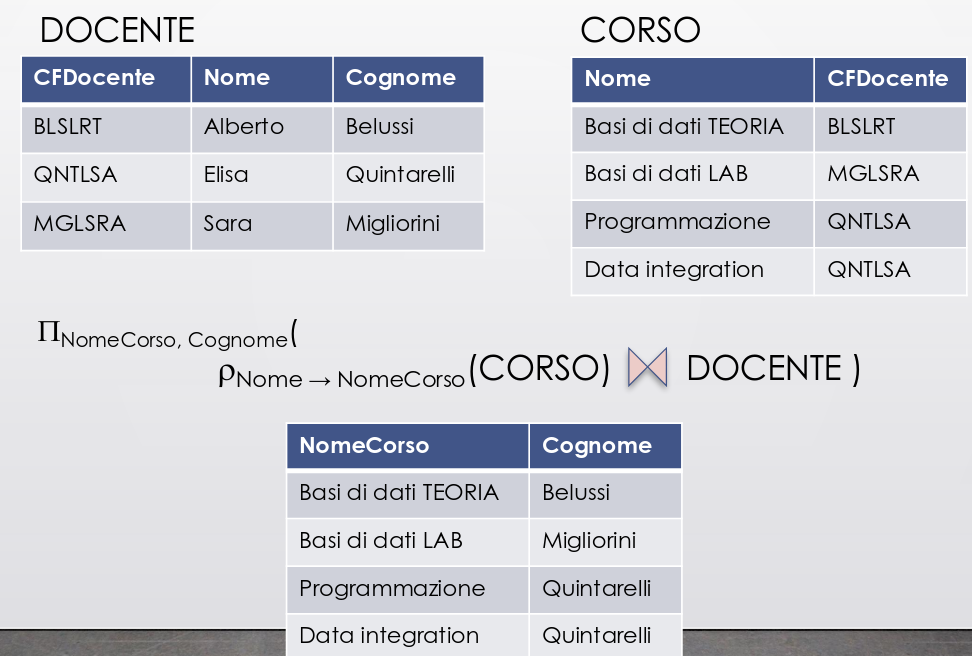
\includegraphics[scale=0.35]{join_example}
\end{center}


Il Join può essere ottenuto tramite un prodotto cartesiano e una selezione imponendo l’uguaglianza su tutti gli attributi in comune:\\

\[\sigma_{\text{NomeCorso = Nome}}(DOCENTE \times CORSO)\]
Il Join si dice completo se ogni tupla della relazione A contribuisce a generare almeno una tupla della relazione risultato, altrimenti si dice incompleto e le tuple che non contribuiscono al risultato si chiamano \textbf{dangling tuples}.

La cardinalità del Join Naturale è, in generale:
\[0 \leq |R1 \bowtie R2| \leq |R1| \cdot |R2|\]
Se il join \`e completo la cardinalit\`a diventa:
\[ max(|R1|, |R2|) \leq |R1 \bowtie R2| \leq |R1| \cdot |R2| \]
Se $X_1 \cap X_2$ \`e una superchiave per $R2$:
\[ 0 \le |R1 \bowtie R2| \leq |R1| \]
Il caso pi\`u classico che ricounduce a questa situazione \`e quando si fa l'uguaglianza tra una \emph{chiave} e una \emph{chiave esportata}, ovvero abbiamo esportato la chiave di $R2$ su $R1$. Se prendo una tupla di $R1$ che ha tra i suoi attributi una \emph{superchiave} di $R2$, si avr\`a al massimo una tupla di $R2$ che va in combinazione con la tupla di partenza di $R1$, perci\`o, \emph{al massimo} la cardinalit\`a sar\`a quella di $R1$. Se $X_1 \cap X_2$ \`e una superchiave di $R2$ ed esiste un \emph{vincolo di integrit\`a referenziale} tra $X_1 \cap X_2$, o una parte di $R1$, e $R2$: $|R1 \bowtie R2| = |R1|$.

\subsection{Theta join ed equi-join}
Nel theta join il predicato di join viene esplicitato, \`e indipendente dallo schema.
Date le relazioni $R1$ e $R2$, rispettivamente di schema $X_1$ e $X_2$, la \textbf{precondizione} al theta join \`e che gli schemi di $R1$ e $R2$ devono essere \emph{disgiunti}: $X_1 \cap X_2 = \varnothing $.
\[ R1 \bowtie_{\theta} R2 = \sigma_{\theta}(R1 \bowtie R2) \]
Dove il join naturale all'interno della selezione funge da \emph{prodotto cartesiano} e $\theta$ \`e un predicato conforme alla sintassi prevista per l'operatore di selezione.
\subsubsection{Esempio}
\texttt{DOCENTE(\underline{CF}, Nome, Cognome)\\
CORSO(\underline{Nome}, Docente)\\
}
Si richiede di produrre l'elenco di tutti i corsi riportando: nome del corso e cognome del docente.
\[ \Pi_{\text{NomeCorso, Cognome}}(\rho_{\text{Nome $\to$ NomeCorso}}(CORSO) {\Large \bowtie \atop \text{\tiny{CF = Docente}}} DOCENTE) \]
Graficamente:
\begin{center}
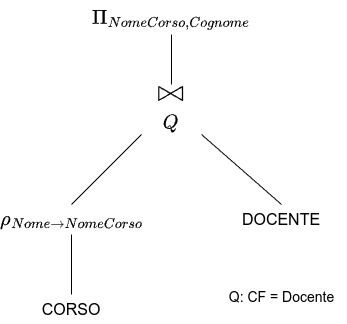
\includegraphics[scale=0.5]{theta_join_example}
\end{center}

\subsubsection{Equi-join}
Il theta join si dice \emph{equi-join} se la condizione $\theta$ \`e una congiunzione di uguaglianze:
\[ R1 {\bowtie \atop A_1 = B_1 \wedge \dots \wedge A_n = B_n} R2 \]

Si noti che \textbf{non esiste} un operatore misto che applica la logica del join naturale per gli attributi comuni e aggiunge la condizione specificata esplicitamente attraverso il predicato $\theta$.

\subsubsection{Propriet\`a dell'equi-join}

Date due relazioni $R1$ e $R2$ di schema $X_1$ e $X_2$, con $X_1 \cap X_2 = \{ C_1, \dots, C_m\}$ con $m > 0$, vale la seguente equivalenza:
\[ R1 \bowtie R2 = \Pi_{X_1 \cup X_2} \left(R1 {\bowtie \atop C_1=C_1' \wedge \dots \wedge C_m=C_m'} \rho_{C_1,\dots,C_m \to C_1', \dots, C_m'}(R2)\right) \]
In questo caso si hanno due relazioni che hanno attributi comuni ($\{ C_1, \dots, C_m\}$) e quindi si devono ridenominare gli attributi di una delle due relaizoni, nell'esempio quelli di $R2$. A questo punto gli schemi sono disgiunti e la condizione del theta-join sar\`a una congiunzione di uguaglianze: $C_1=C_1' \wedge \dots \wedge C_m=C_m'$. Gli attributi che si ottengono nel risultato del theta-join sono la somma degli attributi di $R1$ e di $R2$, cosa che non avviene nel join naturale. Per questo motivo si proietta su $\Pi_{X_1\cup X_2}$, in questo modo l'unione considera gli attributi di tutte e due le relazioni ma esclude i $C_1', \dots, C_m'$ generati nell'espressione.

\subsection{Join esterni}
Consentono di ottenere nel risultato del join tutte le tuple, anche le \textbf{dangling tuples}, di una o di entrambe le relazioni coinvolte nel join, eventualmente estese con valori nulli:
\begin{itemize}
	\item \textbf{left join}: $r_1 \bowtie_{LEFT} r_2$;
	\item \textbf{right join}: $r_1 \bowtie_{RIGHT} r_2$;
	\item \textbf{full join}: $r_1 \bowtie_{FULL} r_2$;
\end{itemize}


\section{Ottimizzazione}
\subsection{Valori nulli}
E’ opportuno estendere l’algebra relazionale affinché possa manipolare anche relazioni che contengono \emph{valori nulli} (NULL). Le operazioni che devono essere raffinate per gestire relazioni che contengono valori nulli sono in particolare \textbf{selezione} e \textbf{join naturale}.\\
Le altre operazioni riportano semplicemente nelle tuple del risultato il valore nullo presente sulle tuple di input.

\subsubsection{Selezione}
Nel caso della \textbf{selezione} abbiamo che la selezione applicata a:
\begin{itemize}
\item $A \theta B$ risulta essere falsa (quindi non seleziona quella determinata tupla) se uno dei due attributi A o B è NULL.
\item $A \theta const$ risulta essere falsa se l'attributo $A$ \`e NULL.
\end{itemize}
Inoltre, si aggiungono le seguenti condizioni atomiche:
\begin{itemize}
\item \texttt{A IS NULL}: \`e una condizione atomica che viene valutata sulla tupla $t$. \`E \textbf{vero} se $t[A]$ \emph{contiene} il valore NULL, altrimenti \`e \textbf{falso}. 
\item \texttt{A IS NOT NULL}: \`e una condizione atomica che viene valutata sulla tupla $t$. \`E \textbf{vero} se $t[A]$ \emph{\underline{non} contiene} il valore NULL, altrimenti \`e \textbf{falso}.
\end{itemize}

\subsubsection{Join naturale}
La condizione di uguaglianza sugli attributi comuni alle due relazioni \`e \textbf{falsa} sulle tuple $t_1$ e $t_2$ se almeno uno degli attributi comuni di $t_1$ o di $t_2$ \`e NULL. Inoltre, il confronto particolare $NULL = NULL$ \`e \textbf{sempre valutato FALSO}.

\subsection{Ottimizzatore}
Ogni espressione DML\footnote{Solitamente specificata in linguaggio dichiarativo} ricevuta dal DBMS viene sottoposta ad un processo di elaborazione, tra cui, anche uno di ottimizzazione. L’ottimizzatore genera un’espressione equivalente all’interrogazione di input e di costo inferiore. quest'ultimo viene valutato in termini di \textbf{dimensione dei risultati intermedi}.
L’ottimizzatore esegue \textbf{trasformazioni di equivalenza} allo scopo di riddurre la dimensione dei risultati intermedi.

\subsubsection{Equivalenza tra espressioni algebriche}

\paragraph{Equivalenza dipendente dallo schema.} Dato uno schema $R$:
$E_1 \equiv E_2$ se $E_1(r) = E_2(r)$ per ogni istanza di $r$ di schema $R$.\\
Esempio:
\[ \Pi_{AB}(R_1) \bowtie \Pi_{AC}(R_2) \equiv_R \Pi_{ABC}(R_1 \bowtie R_2) \]
Con $R=\{R_1(A, B, D), R_2(A, C, E)\}$.

La condizione generale che lo schema deve soddisfare \`e che l'\textbf{unico attributo comune tra $R_1$ e $R_2$ sia $A$}.

\paragraph{Equivalenza assoluta.} \`E indipendente dallo schema.

$E_1 \equiv E_2$ se $E_1 \equiv_R E_2$ per ogni schema $R$ compatibile con $E_1$ ed $E_2$.\\
Esempio:
\[ \Pi_{AB}(\sigma_{A>0}(R_1)) \equiv \sigma_{A>0}(\Pi_{AB}(R1))\]


\subsubsection{Trasformazioni di equivalenza}
Le principali trasformazioni sono quattro. Consideriamo, per gli esempi, il seguente schema relazionale:\\
\texttt{
TRENO(\underline{NumTreno}, OrarioPart, Cat, Dest, OrarioArr)\\
FERMATA(\underline{NumTreno, Stazione}, Orario)
}

Sia $E$ un'espressione di schema $X$, si definiscono le seguenti trasformazioni di equivalenza:
\begin{itemize}
    \item \textbf{Atomizzazione delle selezioni:} una congiunzione di selezioni può essere sostituita da una sequenza di selezioni atomiche.
\[ \sigma_\text{F1 $\wedge$ F2}(E) \equiv \sigma_\text{F1}(\sigma_\text{F2}(E))\] \`E propedeutica ad altre trasformazioni. Non ottimizza se non \`e seguita da altre trasformazioni. \\
Esempio:
\[ \Pi_{\text{NumTreno, OrarioPart}}(\sigma_{\text{Cat='FR' $\wedge$ Stazione='Vicenza'}}(TRENO \bowtie FERMATA) \]
\[ \Large \Rightarrow \]
\[ \Pi_{\text{NumTreno, OrarioPart}}(\sigma_{\text{Cat='FR'}}(\sigma_{\text{Stazione='Vicenza'}}(TRENO \bowtie FERMATA))) \]
\begin{multicols}{2}[Graficamente:]

\begin{center}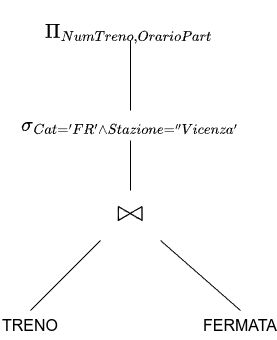
\includegraphics[scale=0.45]{tree_example_transform}\end{center}
\begin{center}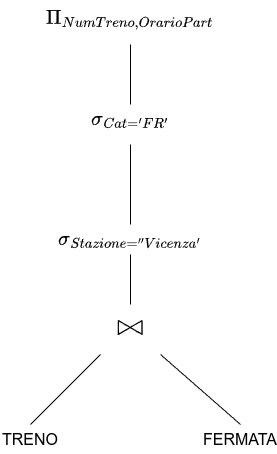
\includegraphics[scale=0.45]{tree_example_atomizz_sel}\end{center}
\end{multicols}
    \item \textbf{Idempotenza delle proiezioni:} una proiezione può essere trasformata in una sequenza di proiezioni che eliminano i vari attributi in varie fasi.
\[ \Pi_\text{A}(E) \equiv \Pi_\text{A}(\Pi_\text{A,B}(E)) \text{ dove }B \subseteq X \]
\`E propedeutica ad altre trasformazioni. Non ottimizza se non \`e seguita da altre trasformazioni. 
\end{itemize}
\newpage
Siano $E_1$ ed $E_2$ espressioni di schema $X_1$ e $X_2$, si definiscono le seguenti trasformazioni di equivalenza:
\begin{itemize}
    \item \textbf{Anticipazione della selezione rispetto al join:} questa espressione vale solo se $F$ conivolge \textbf{solo} gli attributi di $E_2$.
\[ \sigma_{F}(E_1 \bowtie E_2) \equiv_R E_1 \bowtie \sigma_{F}(E_2) \]

Esempio:
\[ \Pi_{\text{NumTreno, OrarioPart}}(\sigma_{\text{Cat='FR' $\wedge$ Stazione='Vicenza'}}(TRENO \bowtie FERMATA) \]
\[ \Large \Rightarrow \]
\[ \Pi_{\text{NumTreno, OrarioPart}}(\sigma_{\text{Cat='FR'}}(TRENO)) \bowtie \sigma_{\text{Stazione='Vicenza'}}(FERMATA)) \]
\begin{multicols}{2}[Graficamente:]

\begin{center}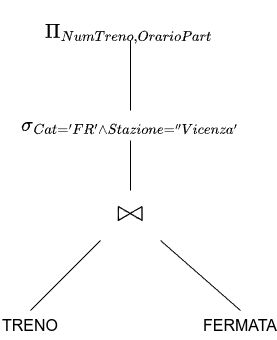
\includegraphics[scale=0.45]{tree_example_transform}\end{center}
\begin{center}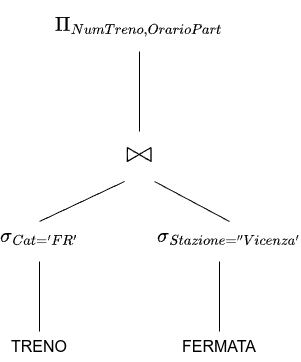
\includegraphics[scale=0.45]{tree_example_anticip_sel}\end{center}
\end{multicols}

    \item \textbf{Anticipazione della proiezione rispetto al Join:} vale solo se Y sono attributi di B e I suoi attributi sono coinvolti nel join.\\
\[\Pi_\text{Y}(A \bowtie B) \equiv A \bowtie(\Pi_\text{Y}(B))\]
Esempio:
\[ \Pi_{\text{NumTreno, OrarioPart}}(\sigma_{\text{Cat='FR' $\wedge$ Stazione='Vicenza'}}(TRENO \bowtie FERMATA) \]
\[ \Large \Rightarrow \]
\[ \Pi_{\text{NumTreno, OrarioPart}}(\Pi_{\text{NumTreno, OrarioPart}}(\sigma_{\text{Cat='FR'}}(TRENO)) \bowtie \Pi_{\text{NumTreno}}(\sigma_{\text{Stazione='Vicenza'}}(FERMATA)) \]
\begin{multicols}{2}[Graficamente:]

\begin{center}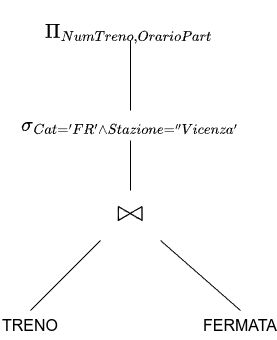
\includegraphics[scale=0.45]{tree_example_transform}\end{center}
\begin{center}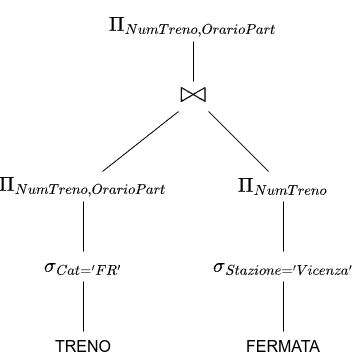
\includegraphics[scale=0.45]{tree_example_anticip_projection}\end{center}
\end{multicols}

    \item Esistono poi altre otimizzazioni minori come l'inglobamento di una selezione in un join (da eseguire solo se non è possibile anticipare la selezione), in questo caso la condizione di selezione sarà assorbita nel \textbf{theta-join}.\\
$$\sigma_\text{F}(A \bowtie B) \equiv A \bowtie_\text{F} B$$
    Infine è bene ricordare anche le trasformazioni con gli operatori insiemistici:\\
$$\sigma_\text{F $\vee$ G}(A) \equiv \sigma_\text{F}(A) \cup \sigma_\text{G}(A)$$
$$\sigma_\text{F $\wedge$ G}(A) \equiv \sigma_\text{F}(A) \cap \sigma_\text{G}(A)$$
    
\end{itemize}

\newpage
\chapter{Calcolo Relazionale}

\`E un linguaggio di interrogazione dichiarativo che specifica le propriet\`a del risultato dell'interrogazione. Esistono due versione del \emph{calcolo relazionale}:
\begin{itemize}
	\item sui domini\footnote{Non presente nel programma.};
	\item \textbf{sulle tuple} (\`e il fondamento teorico del linguaggio \textbf{SQL}).
\end{itemize}

\section{Calcolo relazionale sulle tuple}

Nel calcolo relazionale sulle tuple l'interrogazione viene specificata attraverso una \emph{formula logica con variabili libere}. La formula viene interpretata sul \textbf{contenuto della base di dati} e le variabili assumono come valori le tuple delle relazioni.

Il calcolo relazionale sulle tuple definisce la semantica del linguaggio SQL \emph{semplice}\footnote{Senza operatori aggregati e senza join esterni.}, includendo le interrogazioni nidificate.

\subsection{Formule logiche con variabili libere}
Una variabile si dice \textbf{libera} in una forma logica $F$ se non compare in un \emph{quantificatore} (esistenziale $\exists$ o universale $\forall$) di $F$.

\subsubsection{Esempi:}
\begin{itemize}
\item $F_1(x) \equiv x>3$ $x$ \`e libera.
\item $F_2(x,y) \equiv x>3 \wedge x<6 \wedge y=10$ $x,y$ sono variabili libere.
\item $F_3(x) \equiv x > 0 \wedge \exists y(y<0)$ $x$ \`e libera, $y$ \`e legata.
\item $F_4(x) \equiv x>3 \wedge \exists y(y<x)$ $x$ \`e libera, $y$ \`e legata.
\item $F_5(z) \equiv z<10 \wedge \forall y(y<z)$ $z$ \`e libera, $y$ \`e legata.
\end{itemize}

L'\textbf{interpretazione} \`e la scelta degli insiemi da cui prelevare i valori da sostituire alle variabili. Ad esempio, posso segliere di interpretare le formule nell'insieme degli interi ($\mathbb{Z}$) o nell'insieme dei naturali ($\mathbb{N}$).

\subsubsection{Esempio:}
\[ F_3(x) \equiv x>0 \wedge \exists y(y<0) \]
$F_3(5)$ \`e vera in $\mathbb{N}$? $5 > 0 \to$\texttt{True}, $\exists y(y<0) \to$\texttt{False}. \texttt{True} $\wedge$ \texttt{False} $=$ \texttt{False}, perci\`o la formula \`e falsa.
$F_3(5)$ \`e invece vera nell'insieme dei numeri interi $\mathbb{Z}$. Possiamo dunque notare che al variare dell'insieme di interpretazione, cambia il risultato.
\newpage
\subsection{Sintassi del calcolo relazionale sulle tuple}

Le espressioni del calcolo relazionale sulle tuple hanno la seguente forma:
\[ \{ \text{\texttt{T}} | \text{\texttt{L}} | \text{\texttt{F}} \} \]
\begin{itemize}
\item \textbf{Target list} \texttt{T} $\to$ corrisponde alla \texttt{SELECT} dell'SQL. Definisce lo \emph{schema della relaziona risultato} e come le tuple risultato si ottengono dalle variabili libere.
\item \textbf{Range list} \texttt{L} $\to$ corrisponde a \texttt{FROM} dell'SQL. Definisce le \emph{variabili libere} e le collega alle relazioni della base di dati coinvolte nell'interrogazione.
\item \textbf{Formula} \texttt{F} $\to$ corrisponde a \texttt{WHERE} dell'SQL. Specifica la condizione che deve essere soddisfatta dalle variabili libere, vale a dire dalle tuple coinvolte nell'interrogazione.
\end{itemize}

\subsubsection{Target list}
\texttt{T} \`e una lista di elementi separati da virgole $e_1, \dots, e_n$ dove ogni elemento $e_i$ pu\`o essere:
\begin{itemize}
	\item \texttt{Y: x. (Z)}, dove \texttt{Y} e \texttt{Z} sono sequenze di attributi con la stessa cardinalit\`a e \texttt{x} \`e una \emph{variabile libera}.
	\item \texttt{x. (Z)}, dove \texttt{Z} \`e una sequenza di attributi e \texttt{x} \`e una \emph{variabile libera} (equivale a \texttt{Z: x. (Z)}). 
	\item \texttt{x. *}, dove \texttt{x} \`e una \emph{variabile libera}; in questo caso gli attributi sono esattamente tutti quelli della relazione associata alla variabile \texttt{x} nella \textbf{range list} \texttt{L}.
\end{itemize}

\subsubsection{Range list}
\texttt{L} \`e una lista di elementi separati da virgole $r_1, \dots, r_m$ dove ogni elemento $r_i$ \`e strutturato come \texttt{x\textsubscript{j}(R)}, in cui \texttt{R} rappresenta una relazione, o tabella, della base di dati. (La variabile $x_j$ prender\`a come valori le tuple della tabella $R$ quando si va a valutare la formula).
Il numero degli elementi \textbf{deve corrispondere} al numero di variabili libere.

\subsubsection{Formula}
\texttt{F} pu\`o essere 
\begin{itemize}
	\item una \textbf{formula atomica}, del tipo \texttt{x.A $\theta$ c} oppure \texttt{x\textsubscript{1}.A\textsubscript{1} $\theta$ x\textsubscript{2}.A\textsubscript{2}}, dove \texttt{x, x\textsubscript{1}, x\textsubscript{2}} sono variabili, \texttt{A, A\textsubscript{1}, A\textsubscript{2}} sono attributi, \texttt{c} \`e una costante e $\theta \in \{ =, \ne, >, <, \le, \ge\}$. Nelle formule atomiche \emph{tutte le variabili} sono \emph{LIBERE}.
	\item oppure una \textbf{formula non atomica}:
	\begin{itemize}
		\item se $f_1$ e $f_2$ sono formule, allora anche $f_1 \wedge f_2$, $f_1 \vee f_2$, $\neg f_1$, e $\neg f_2$ lo sono.
		\item Se $f$ \`e una formula, allora anche $\forall x(R) (f)$ e $\exists x (R) (f)$ lo sono. 
	\end{itemize}
	Nelle formule $\forall x (f)$ e $\exists x(f)$, $x$ \`e una variabile \emph{LEGATA}, mentre tutte le altre variabili sono libere o legate se lo sono in $f$.
Inoltre, le congiunzioni, disgiunzioni e la negazione non cambiano l'insieme delle variabili \emph{LIBERE} o \emph{LEGATE} di una formula.
\end{itemize}

\subsection{Semantica: interpretazione delle formule}

Le formule vengono interpretate sull'istanza corrente della
\begin{itemize}
\item base di dati $db = \{r_1, \dots, r_n\}$ 
\item di schema $S = \{R_1(X_1), \dots, R_n(X_n)\}$
\end{itemize}
Ogni formula contiene un certo numero di variabili libere:
\begin{itemize}
\item $f(x_1, \dots, x_2)$
\end{itemize}

Data una ennupla di tuple $t_1, \dots, t_n$, tale ennupla rende vera la formula se, quando sostituisco le tuple $t_1, \dots, t_n$ alle variabili libere $x_1, \dots, x_n$, tale sostituzione soddisfa la formula.

\subsubsection{Formule atomiche}
\begin{itemize}
\item \texttt{x\textsubscript{1}.A\textsubscript{1} $\theta$ x\textsubscript{2}.A\textsubscript{2}} \`e vera sulle tuple $(t_1, t_2)$, se il confronto \texttt{t\textsubscript{1}[A\textsubscript{1}] $\theta$ t\textsubscript{2}[A\textsubscript{2}]} \`e soddisfatto.
\item \texttt{x\textsubscript{1}.A\textsubscript{1} $\theta$ c} \`e vera sulla tupla $t_1$, se il confronto \texttt{t\textsubscript{1}[A\textsubscript{1}] $\theta$ c} \`e soddisfatto.
\end{itemize}

\subsubsection{Formule non atomiche}

Le formule $f_1 \wedge f_2$, $f_1 \vee f_2$, $\neg f_1$, $\neg f_2$ sono vere secondo le usuali definizioni dei connettivi logici (tabelle di verit\`a).

\subsubsection{Formule con quantificatori}

\begin{itemize}
\item $\exists x(R_i)(f)$ con variabili libere $(x_1, \dots, x_q)$ \`e vera sulle tuple $(t_1, \dots, t_q)$, se \textbf{esiste almeno} una tupla $t\in r_1$\footnote{Istanza di $R_i$} tale che $f$ \`e vera quando si sostituiscono le tuple $(t, t_1, \dots, t_q)$ alle variabili $(x, x_1, \dots, x_q)$.
\item $\forall x(R_i)(f)$ con variabili libere $(x_1, \dots, x_q)$ \`e vera sulle tuple $(t_1, \dots, t_q)$, se \textbf{per ogni} tupla $t\in r_i$, $f$ \`e vera quando si sostituiscono le tuple $(t, t_1, \dots, t_q)$ alle variabili $(x, x_1, \dots, x_q)$.
\end{itemize}


\subsection{Semantica di una interrogazione}

Interpretazone di un'espressione del calcolo come interrogazione. Struttura:
\[ Q= \{Y_1:x_1 . (Z_1),\dots,Y_k:x_k . (Z_k) | x_1(R_1), \dots, x_n(R_n) | f(x_1, \dots, x_n) \} \]

La valutazione dell'interrogazione $Q$ produce una relazione risultato $R$ dove:
\begin{itemize}
\item Lo schema di $R$ \`e $Y = Y_1 \cup \dots \cup Y_k$
\item $R$ contiene tutte le tuple $t$ su $Y$ tali che esiste una ennupla di tuple $(t_1, \dots, t_n) \in R_1 \times \dots \times R_n$, che generano $t$ e che sostituite alle variabili libere $(x_1, \dots, x_n)$ rendono vera $f$.
\end{itemize}

\subsection{Osservazioni}
Il calcolo relazionale sulle tuple \textbf{non \`e equivalente all'algebra relazionale} e non \`e equivalente al calcolo relazionale sui domini, in quanto l'unione di due relazioni non \`e rappresentabile nel calcolo relazionale sulle tuple.

\`E invece possibile rappresentare nel calcolo relazionale sulle tuple sia l'intersezione che la differenza tra due relazioni.

\subsection{Operatori insiemistici nel calcolo relazionale sulle tuple}

\subsubsection{Intersezione}
L'intersezione tra due relazioni $R_1$ e $R_2$ di schema $X=(A_1, \dots, A_n)$ si ottiene:
\[ R_1 \cap R_2 \equiv \{ x.* | x(R_1), y_2(R_2) | x.A_1 = y.A_1 \wedge \dots \wedge x.A_n = y.A_n \} \]
Possiamo ottenere lo stesso risultato utilizzando il quantificatore esistenziale ($\exists$):
\[ R_1 \cap R_2 \equiv \{ x.* | x(R_1)| \exists y(R_2)(x.A_1 = y.A_1 \wedge \dots \wedge x.A_n = y.A_n) \} \]

\subsubsection{Differenza}

La differenza tra due relazioni $R_1$ e $R_2$ di schema $X=(A_1, \dots, A_n)$ si scrive:
\[ R_1 - R_2 \equiv \{x.* | x(R_1) | \neg \exists y(R_2) (x.A_1=y.A_1 \wedge \dots \wedge x.A_n = y.A_n) \} \]

\subsubsection{Unione}

L'unione tra due relazioni $R_1$ e $R_2$ di schema $X=(A_1, \dots, A_n)$ \textbf{\color{red}{non \`e esprimibile}} in quanto \textbf{non \`e possibile associare una variabile libera a pi\`u relazioni della base di dati}.

Notare che $\{ x_1.*, x_2.* | x_1(R_1), x_2(R_2) | true \}$ genera il \emph{prodotto cartesiano} e non l'unione.

\subsection{Esercizi}

Schema:\\
\texttt{TRENO(\underline{Num}, Cat, Part, Arr, Dest)\\
FERMATA(\underline{Treno, Staz}, Orario)}

\paragraph{Q\textsubscript{0}: Trovare il numero e l'ora di partenza dei treni Freccia Rossa con destinazione Milano Centrale.}

\[ Q_0: \{t.(\text{\texttt{Num, Part}}) |t(\text{\texttt{TRENO}}) | t.\text{\texttt{Cat='FR'}} \wedge t.\text{\texttt{Dest='Milano Centrale'}} \} \]

\paragraph{Q\textsubscript{1}: Trovare l'elenco di tutte le fermate dei treni regionali, riportando nel risultato il numero del treno e la stazione di fermata.}

\[ Q_1: \{f.(\text{\texttt{Treno, Staz}}) | t(\text{\texttt{TRENO}}), f(\text{\texttt{FERMATA}}) | t.\text{\texttt{Cat='REG'}} \wedge t.\text{\texttt{Num}} = f.\text{\texttt{Treno}} \} \]

\paragraph{Q\textsubscript{2}: Trovare l'elenco di tutti i treni Freccia Rossa che fermano a Venezia Mestre riportando: il numero del treno, l'orario di partenza e l'orario di arrivo.}

\[ Q_2: \{t.(\text{\texttt{Num, Part}}), f.(\text{\texttt{Orario}}) | t(\text{\texttt{TRENO}}), f(\text{\texttt{FERMATA}}) |t.\text{\texttt{Num}} = f.\text{\texttt{Treno}}\wedge f.\text{\texttt{Staz='Venezia Mestre'}} \wedge t.\text{\texttt{Cat='FR'}} \} \]

\paragraph{Q\textsubscript{3}: Trovare la destinazione e l'orario di partenza dei treni che fermano a Padova.}

\[ Q_3: \{t.(\text{\texttt{Dest, Part}})| t(\text{\texttt{TRENO}}), f(\text{\texttt{FERMATA}}) |t.\text{\texttt{Num}} = f.\text{\texttt{Treno}}\wedge f.\text{\texttt{Staz='Padova'}}\} \]
oppure 
\[ Q_3: \{t.(\text{\texttt{Dest, Part}})| t(\text{\texttt{TRENO}}) | \exists f(\text{\texttt{FERMATA}}) (t.\text{\texttt{Num}} = f.\text{\texttt{Treno}}\wedge f.\text{\texttt{Staz='Padova'}})\} \]

\paragraph{Q\textsubscript{4}: Trovare la destinazione e l'orario di partenza dei treni che \underline{non fermano} a Padova.}

In questo caso non possiamo mettere \texttt{FERMATA} nella target list. Questa interrogazione non pu\`o essere ottenuta attraverso un join, ma si ottiene con una differenza.

\[ Q_4: \{t.(\text{\texttt{Dest, Part}})| t(\text{\texttt{TRENO}}) | \neg\exists f(\text{\texttt{FERMATA}}) (t.\text{\texttt{Num}} = f.\text{\texttt{Treno}}\wedge f.\text{\texttt{Staz='Padova'}})\} \]

\subsection{Calcolo relazionale sulle tuple}

Il calcolo relazionale sulle tuple \`e equivalente al linguaggio di interrogazione adottato dallo standard SQL2 se consideriamo la forma base dell'interrogazione SQL senza operatori aggregati e raggrupamenti. 

L'espressione del calcolo \texttt{\{ T | L | F\}} \`e in diretta corrispondenza con la forma base delle interrogazioni SQL.
\begin{center}
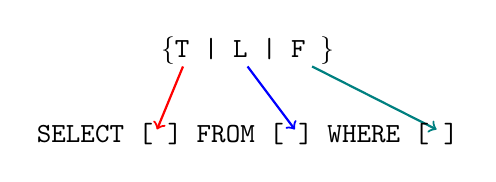
\begin{tikzpicture}
\node at (0,5) [above] {\texttt{\{T | L | F \}}};
\draw[->][red][thick] (-0.82,5.1) -- (-1.15, 4.3); 
\draw[->][blue][thick] (0,5.1) -- (0.60,4.3);
\draw[->][teal][thick] (0.82,5.1) -- (2.4,4.3);
\node at (0,4.5) [below] {\texttt{SELECT [ ] FROM [ ] WHERE [ ]}}; 
\end{tikzpicture}
\end{center}

\subsubsection{Uso dei quantificatori}

Nelle formule del calcolo \`e possibile esprimere condizioni attravarso l'uso di quantificatori ($\exists$ e $\forall$).

Le espressioni che possono essere specificate attraverso i quantificatori corrispondono in SQL a clausole \texttt{WHERE} nelle quali compaiono \textbf{predicati complessi che richiedono interrogazioni nidificate}.

\subsubsection{Esempio}
Schema:\\
\texttt{TRENO(\underline{Num}, Cat, Part, Arr, Dest)\\
FERMATA(\underline{Treno, Staz}, Orario)}

\paragraph{Q\textsubscript{5}: Trovare il numero e la categoria dei treni che fermano a Vicenza e fermano a Padova dopo le 20:30.}

\[ Q_5: \{\text{\texttt{Numero, Categoria}}:t.(\text{\texttt{Num, Cat}})| t(\text{\texttt{TRENO}}) | \exists f_1(\text{\texttt{FERMATA}}) (t.\text{\texttt{Num}} = f_1.\text{\texttt{Treno}}\wedge f_1.\text{\texttt{Staz='Vicenza'}\\})\]
\[ \wedge \exists f_2(\text{\texttt{FERMATA}}) (t.\text{\texttt{Num}} = f_2.\text{\texttt{Treno}}\wedge f_2.\text{\texttt{Staz='Padova'}} \wedge f_2.\text{\texttt{Orario > 20:30}})\} \]

\`E possibile eliminare il quantificatore esistenziale nell'esempio $Q_5$, perch\'e non \`e negato. In altre parole, questa interrogazione \`e possibile farla in \emph{algebra relazionale} utilizzando due join. Alternativa:

\[ Q_5: \{\text{\texttt{Numero, Categoria}}:t.(\text{\texttt{Num, Cat}})| t(\text{\texttt{TRENO}}), f_1(\text{\texttt{FERMATA}}), f_2(\text{\texttt{FERMATA}})| \]
\[ t.\text{\texttt{Num}} = f_1.\text{\texttt{Treno}}\wedge f_1.\text{\texttt{Staz='Vicenza'}} \wedge t.\text{\texttt{Num}} = f_2.\text{\texttt{Treno}} \wedge f_2.\text{\texttt{Staz='Padova'}} \wedge f_2.\text{\texttt{Orario > 20:30}}\} \]

\subsection{Esercizi}
Schema:\\
\texttt{TRENO(\underline{Num}, Cat, Part, Arr, Dest)\\
FERMATA(\underline{Treno, Staz}, Orario)}


\paragraph{Q\textsubscript{6}: Trovare per ogni stazione il numero dell'ultimo treno che ferma in quella stazione.}

\[ Q_6: \{f.(\text{\texttt{Treno, Staz}})| f(\text{\texttt{FERMATA}}) | \neg\exists g(\text{\texttt{FERMATA}}) (g.\text{\texttt{Staz}} = f.\text{\texttt{Staz}}\wedge g.\text{\texttt{Orario}} > f.\text{\texttt{Orario}} )\]

Che equivale all'espressione con il quantificatore universale $\forall$:


\[ Q_6: \{f.(\text{\texttt{Treno, Staz}})| f(\text{\texttt{FERMATA}}) | \forall g(\text{\texttt{FERMATA}}) (g.\text{\texttt{Staz}} = f.\text{\texttt{Staz}}\Rightarrow g.\text{\texttt{Orario}} \le f.\text{\texttt{Orario}} )\]



\paragraph{Q\textsubscript{7}: Trovare l'elenco di tutte le stazioni dove fermano tutti i treni con destinazione Venezia SL.}


\[ Q_7: \{f.(\text{\texttt{Staz}})| f(\text{\texttt{FERMATA}}) | \forall t(\text{\texttt{TRENO}}) (t.\text{\texttt{Dest='Venezia SL'}} \Rightarrow \exists g(FERMATA)(t.\text{\texttt{Num}} = g.\text{\texttt{Treno}} \wedge f.\text{\texttt{Staz}} = g.\text{\texttt{Staz}} ))\]

In questo caso non \`e possibile in alcun modo eliminare il quantificatore universale.

\paragraph{Q\textsubscript{8}: Trovare per ogni treno regionale il treno freccia rossa immediatamente successivo con la stessa de
stinazione, riportando nel risultato il numero e l'orario di partenza dei due treni insieme alla loro destinazione.}


\[ Q_8: \{\text{\texttt{Num\_REG, Part\_REG}} : t.(\text{\texttt{Num, Part}}),\text{\texttt{Num\_FR, Part\_FR}} : p.(\text{\texttt{Num, Part}}) | t(\text{\texttt{TRENO}}), p(\text{\texttt{TRENO}}) |\]
\[ t.\text{\texttt{Cat='REG'}} \wedge p.\text{\texttt{Cat='FR'}} \wedge t.\text{\texttt{Dest}} = p.\text{\texttt{Dest}} \wedge t.\text{\texttt{Part}} < p.\text{\texttt{Part}} \wedge \neg\exists q(\text{\texttt{TRENO}})(t.\text{\texttt{Dest}} = q.\text{\texttt{Dest}} \wedge q.\text{\texttt{Cat='FR'}} \wedge \]
\[t.\text{\texttt{Part}} < q.\text{\texttt{Part}} \wedge q.\text{\texttt{Part}} < p.\text{\texttt{Part}} )\]
Possiamo scrivere questa interrogazione in Algebra:
\begin{center}
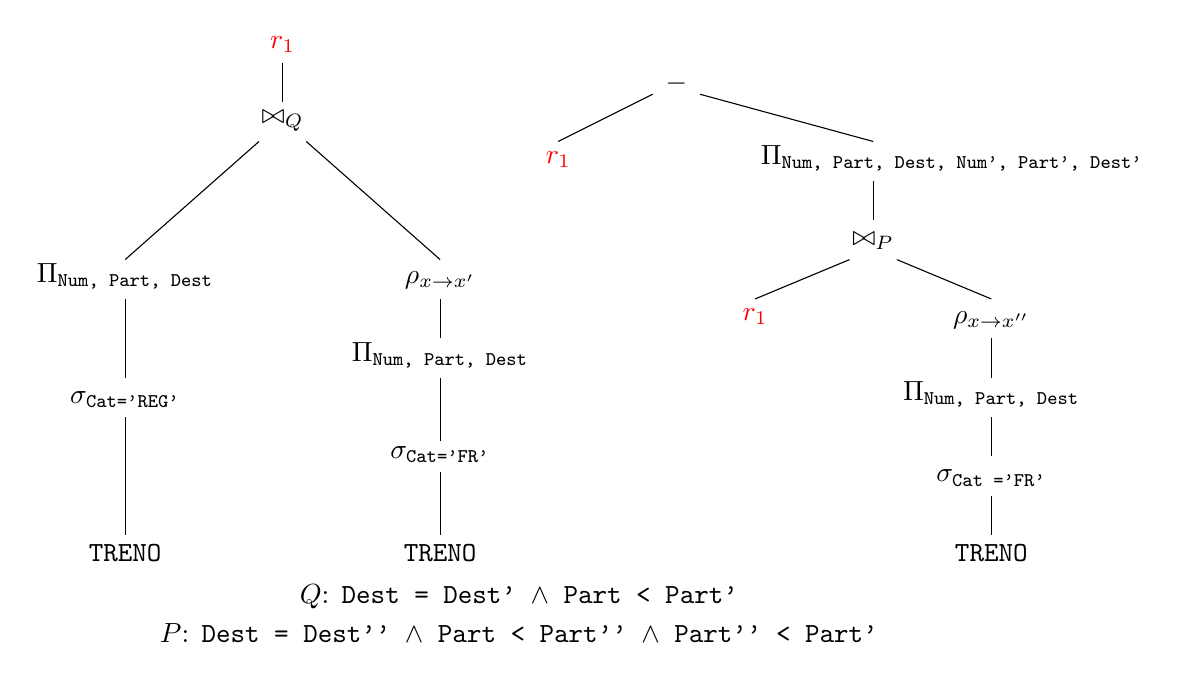
\begin{tikzpicture}
\node at (3,7) [above][red] {$r_1$};
\draw (3,6.5) -- (3,7);
\node at (3,6) [above] {$\Large \bowtie_{Q}$};
% Ramo sinistro
\draw (2.7,6) -- (1,4.5);
\node at (1,4) [above] {$\Pi_{\text{\texttt{Num, Part, Dest}}}$};
\draw (1,4) -- (1,3);
\node at (1, 2.5) [above] {$\sigma_{\texttt{Cat='REG'}}$};
\draw (1,2.5) -- (1,1);
\node at (1,1) [below] {\texttt{TRENO}};
% Ramo destro
\draw (3.3,6) -- (5,4.5);
\node at (5,4) [above] {$\rho_{x \to x'}$};
\draw (5,4) -- (5,3.5);
\node at (5,3) [above] {$\Pi_{\texttt{Num, Part, Dest}}$};
\draw (5,3) -- (5,2.2);
\node at (5,1.8) [above] {$\sigma_{\texttt{Cat='FR'}}$};
\draw (5,1.8) -- (5,1);
\node at (5,1) [below] {\texttt{TRENO}};
\node at (6, 0.5) [below] {$Q$: \texttt{Dest = Dest' $\wedge$ Part < Part'}}; 

% Differenza

\node at (8,6.5) [above] {$\Large -$};
% Ramo sinistro
\draw (7.7,6.6) -- (6.5,6);
\node at (6.5,6) [below][red] {$r_1$};
% Ramo destro
\draw (8.3, 6.6) -- (10.5, 6);
\node at (11.5, 5.5) [above] {$\Pi_{\texttt{Num, Part, Dest, Num', Part', Dest'}}$};
\draw (10.5,5.5) -- (10.5,5);
\node at (10.5, 4.5) [above] {$\Large \bowtie_{P}$};
% Ramo sinistro
\draw (9,4) -- (10.2, 4.5);
\node at (9,4) [below][red] {$r_1$};

% Ramo destro
\draw (10.8, 4.5) -- (12, 4);
\node at (12, 3.5) [above] {$\rho_{x \to x''}$};
\draw (12,3.5) -- (12, 3);
\node at (12,2.5) [above] {$\Pi_{\texttt{Num, Part, Dest}}$};
\draw (12, 2.5) -- (12, 2);
\node at (12, 1.5) [above] {$\sigma_{\texttt{Cat ='FR'}}$};
\draw (12,1.5) -- (12,1);
\node at (12, 1) [below] {\texttt{TRENO}};
\node at (6, 0) [below] {$P$: \texttt{Dest = Dest'' $\wedge$ Part < Part'' $\wedge$ Part'' < Part'}};
\end{tikzpicture}
\end{center}

\chapter{Interrogazioni nei sistemi document-based}

\section{Linguaggi di interrogazione nei sistemi NoSQL}

Nei sistemi NoSQL spesso non sono disponibili veri e propri linguaggi di interrogazione come nei sistemi relazionali. Solo i sistemi \textbf{document-based} forniscono strumenti simili ad algebra e calcolo relazionale per l'accesso ai dati. Due esempi sono:
\begin{itemize}
\item \textbf{Couchbase}, che fornisce il linguaggio SQL++, simile all'SQL e dichiarativo.
\item \textbf{MongoDB}, che fornisce una \textbf{serie di operatori} che consentono di scrivere complesse espressioni algebriche (pipeline) per estrarre dati dalle collezioni di documenti.
\end{itemize}

\subsubsection{Sistemi document-store}
\begin{multicols}{2}
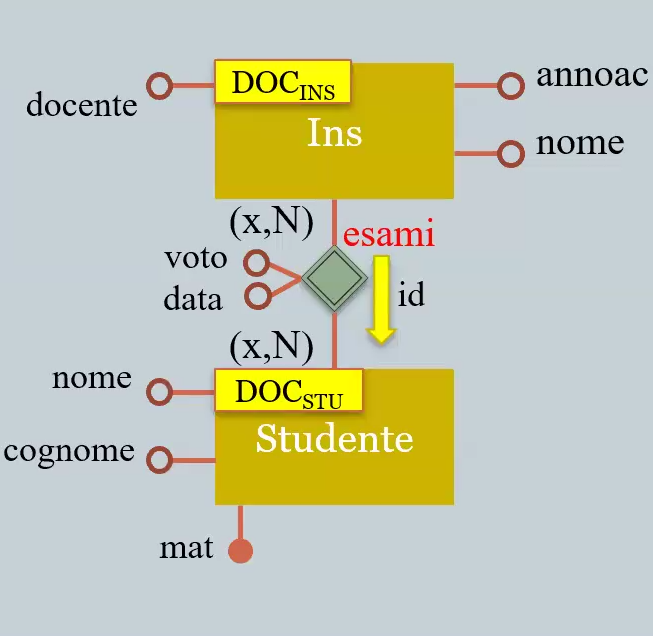
\includegraphics[scale=0.4]{document_store_example} 
\newcolumn
\begin{lstlisting}
		DOC_Ins
{
 _id: autogen
 nome: String
 annoac: String
 docente: String
}

		DOC_Stu
{
 _id: autogen
 nome: String
 cognome: String
 esami: [{Ins_id: integer
 			voto: integer
 			data: date},
 			...]
}
\end{lstlisting}
\end{multicols}
\newpage
\subsection{Approccio MongoDB}

Buona parte del linguaggio di interrogazione di MongoDB \`e realizzato attraverso il metodo \texttt{find}. Interrogazione sull'esempio sopra riportato:

\begin{lstlisting}
db.studenti.insertMany([
{_id: ``VR00010'', nome: ``Mario'', cognome: ``Rossi''
 esami: [{ins: ``Basi di dati'', voto: 22, data: ``1/7/2016'' },
 	{ins: ``Algebra'', voto: 26, data: ``5/7/2015'' }] }
{_id: ``VR00011'', nome: ``Maria'', cognome: ``Bianchi''
 esami: [{ins:' ``Algebra'', voto: 30, data: ``1/7/2016'' }]}
]);
\end{lstlisting}

\subsubsection{Interrogazioni semplici}
Il sistema nasce inizialmente per fare solo questo tipo di interrogazioni. Le interrogazioni semplici sono quelle \emph{monocollezione}.
\begin{itemize}
\item Trovare tutti gli studenti:
\begin{lstlisting}
db.studenti.find( {} )
\end{lstlisting}
\item Trovare tutti gli studenti di cognome \emph{Rossi}:
\begin{lstlisting}
db.studenti.find( {cognome: ``Rossi''} )
\end{lstlisting}
\item Trovare tutti gli studenti di cognome ``Rossi'' e nome ``Mario'':
\begin{lstlisting}
db.studenti.find( {cognome: ``Rossi'', nome: ``Mario''} )
\end{lstlisting}
\item Trovare tutti gli studenti di cognome ``Rossi'' o ``Bianchi'':
\begin{lstlisting}
db.studenti.find( {cognome: {$in:[``Rossi'', ``Bianchi''] }} )
\end{lstlisting}
\end{itemize}

\subsubsection{Operatori logici e di confronto}

\begin{itemize}
\item \texttt{\$and}: unisce due clausole con un and logico e restituisce tutti i documenti che rispettano entrambe le clausole.
\begin{lstlisting}
{$and: [{Esami.voto: {$gte: 21}}, {Esami.voto: {$lte: 26}} ]}
\end{lstlisting}
\item \texttt{\$not}: inverte l'effetto dell'espressione di interrogazione e restituisce i documenti che \textbf{non rispettano} la clausola.
\item \texttt{\$nor}: unisce le clausole con un nor logico e restituisce i documenti che \textbf{non rispettano} entrambe le clausole.
\item \texttt{\$or}: unisce le clausole con un or logico e restituisce i documenti che rispettano almeno una delle due clausole.
\begin{lstlisting}
{$or: [{Cognome: ``Rossi''}, {Cognome: ``Bianchi''}]}
\end{lstlisting}
\item \texttt{\$eq}: restituisce i valori uguali ad un valore specificato.
\item \texttt{\$gt}/\texttt{\$lt}: restituisce i valori maggiori/minori di un valore specificato.
\item \texttt{\$gte}/\texttt{\$lte}: restituisce i valori maggiori o uguali/minori o uguali di un valore specificato.
\item \texttt{\$in}: corrispondenza con qualsiasi valore all'interno di un dato array.
\item \texttt{\$ne}: corrispondenza con tutti i valori diversi da un valore specificato.
\item \texttt{\$nin}: corrispondenza con nessuno dei valori specificati in un array.
\end{itemize}

\subsubsection{Interrogazioni su dati incapsulati}

\begin{itemize}
\item Trovare tutti gli studenti che hanno registrato \emph{almeno un esame} con voto 30:
\begin{lstlisting}
db.studenti.fint( {esami.voto: 30} )
\end{lstlisting}
\item Trovare tutti gli studenti che hanno registrato \emph{almeno un esame} con voto maggiore di 22:
\begin{lstlisting}
db.studenti.find( {esami.voto: { $gt: 22 } } )
\end{lstlisting}
\end{itemize}

\subsubsection{Interrogazioni con proiezione}

La proiezione permette di definire qual \`e la struttura del documento risultato.\\
Esempi:
\begin{itemize}
\item Trovare il cognome degli studenti di nome ``Mario'':
\begin{lstlisting}
db.studenti.find( {nome: ``Mario''}, {cognome: 1} )
\end{lstlisting}
\item Trovare il cognome degli studenti di nome ``Mario'' escludendo il campo \texttt{\_id}:
\begin{lstlisting}
db.studenti.find( {nome: ``Mario''}, {cognome: 1, _id: 0} )
\end{lstlisting}
\item Trovare la matricola e i voti di tutti gli studenti:
\begin{lstlisting}
db.studenti.find( { }, {_id: 1, esami.voto: 1} )
\end{lstlisting}
\end{itemize}

\subsubsection{Interrogazioni con join}

Per eseguire un join tra due collezioni di documenti \`e necessario usare l'operazione \texttt{\$lookup} di \texttt{aggregate}. Questo tipo di interrogazioni non sono consigliate dal sistema. 

\begin{multicols}{2}[Esempio:]
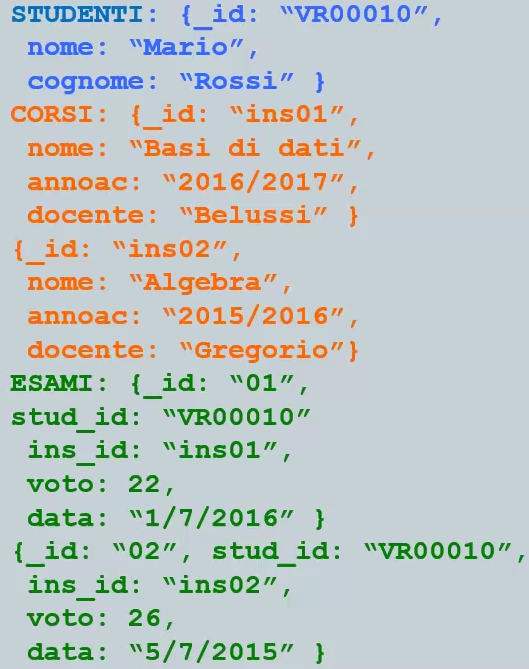
\includegraphics[scale=0.5]{document_store_example_2}
\newcolumn

\begin{lstlisting}
db.STUDENTI.aggregate([
  { $lookup:
	 { from: ESAMI,
	   localField: _id,
	   foreignField: stud_id,
	   as: ``esami_fatti''
	 }
  }
])
\end{lstlisting}

Si vuole, per esempio, incapsulare dentro a \color{blue}\textbf{STUDENTI} \color{black}i suoi esami. Non si generano le coppie, ma una \textbf{nuova propriet\`a} dentro \color{blue}\textbf{STUDENTI} \color{black}che conterr\`a tutte le istanze di \color{green}\textbf{ESAMI} \color{black} che si agganciano a quello studente.\\Risultato:

\begin{lstlisting}
{ _id: ``VR00010'',
 nome: ``Mario'',
 cognome: ``Rossi'',
 ``esami_fatti'': [
 	{_id: ``01'', stud_id: ``VR00010'',
 	 ins_id: ``ins01'', voto: 22, 
 	 data: ``1/7/2016'' },
   {_id: ``02'', stud_id: ``VR00010'', 
    ins_id: ``ins02'', voto: 26, 
    data: ``5/7/2015'' } ]
}
\end{lstlisting}


\end{multicols}




































\end{document}
